\documentclass[
11pt,
usepdftitle=false,
aspectratio=169,
xcolor={table,usenames,dvipsnames},
%handout,
]{beamer}

\usetheme[nototalframenumber,nosectiontitlepage,foot,logo,url]{uibk}
\usepackage[utf8]{inputenc}
\usepackage{amsmath,amssymb,alltt}
\usepackage{xcolor}
\usepackage[english]{babel}
\usepackage{stmaryrd}
\usepackage{wasysym}
\usepackage{pifont}
\RequirePackage{etex}
\usepackage{tikz}
\usetikzlibrary{backgrounds}
\usetikzlibrary{fit}
\usetikzlibrary{matrix}
\usetikzlibrary{shapes.symbols}
\usetikzlibrary{shapes.callouts}
\usetikzlibrary{shapes.geometric}
\usetikzlibrary{shapes.arrows}
\usetikzlibrary{arrows}
\usetikzlibrary{arrows.meta}
\usetikzlibrary{trees}
\usetikzlibrary{shadows}
\usetikzlibrary{shadings}
\usetikzlibrary{automata}
\usetikzlibrary{decorations.pathmorphing}
\usetikzlibrary{decorations.pathreplacing}
\usetikzlibrary{calc}
\usetikzlibrary{fadings}
\usetikzlibrary{positioning}
\usetikzlibrary{mindmap}
\usetikzlibrary{through}
% \usepackage{mathpartir}
% \usepackage{graphicx}
% \usepackage{proof}
\usepackage{xargs}
% \usepackage{paralist}
% \usepackage{multirow}
\usepackage{listings}
% \usepackage{turnstile}
\usepackage{xfrac}
\usepackage[most]{tcolorbox}
% \usepackage{arydshln}

%\usepackage{newtxmath}
\usepackage{amsmath,amssymb,alltt}
% \usepackage{hyperref}
\usepackage{nccmath}
% \usepackage{amsthm}
% \usepackage[utf8]{inputenc}
% \usepackage[T1]{fontenc}
\usepackage{mathtools}
% % \usepackage{mathrsfs}

% \usepackage[english]{babel}
% \usepackage{listings}
% %\usepackage{fontspec}
\usepackage{pifont}
% \usepackage{xfrac}
\usepackage{colortbl,booktabs}

\usepackage{pgfplots}
\pgfplotsset{compat=1.7}

\usepackage{caption}
\captionsetup[table]{justification=raggedright,singlelinecheck=false}
% \usepackage{forest}
\usepackage{general}
\usepackage{code}
\usepackage{tctschematic}
\usepackage{pars}
\usepackage{while}
\usepackage{algpseudocode}
\usepackage{xfp}
\usepackage{slides}

\setbeamertemplate{sidebar right}{}
\setbeamertemplate{sections/subsections in toc}[ball unnumbered]
\setbeamersize{text margin left=5mm,text margin right=5mm}
\setbeamertemplate{itemize items}[circle]
\setbeamertemplate{enumerate items}[square]
\setbeamertemplate{qed symbol}{\vrule width 1.5ex height 1.5ex depth 0pt}

\newcommand{\DARKGREEN}[1]{{\color{green!30!black}#1}}
%\newcommand{\BLACK}[1]{{\color{black}#1}}
%\newcommand{\RED}[1]{{\alert{#1}}}
\newcommand{\DARKRED}[1]{{\color{amaranth!50!black}#1}}
\newcommand{\DARKBLUE}[1]{{\color{blue!50!black}#1}}
\newcommand{\BLUE}[1]{{\color{airforceblue}#1}}
%\newcommand{\MAGENTA}[1]{{\color{magenta}#1}}
%\newcommand{\YELLOW}[1]{{\color{yellow}#1}}
%\newcommand{\WHITE}[1]{{\color{white}#1}}
\definecolor{darkgray}{rgb}{0.31,0.31,0.33}
%\newcommand{\GRAY}[1]{{\color{darkgray}#1}}
\definecolor[named]{darkviolet}{HTML}{1b0160}
\definecolor[named]{keyword}{HTML}{e0004a} %TODO: make c/b friendlier
%\definecolor[named]{keyword}{rgb}{0.99,0.78,0.07}
\definecolor[named]{constructor}{HTML}{009304}
\definecolor[named]{warmYellow}{rgb}{0.99,0.78,0.07}
\definecolor[named]{extension}{HTML}{1e88e5}% coin, tick ("probabilistic extension"), nondeterminism
\definecolor[named]{basic}{HTML}{1b0160}

\newcommand{\red}[1]{{\color{orange} #1}} % colorblind friendly
\newcommand{\blue}[1]{{\color{blue!80} #1}}
\newcommand{\green}[1]{{\color{ForestGreen} #1}}

% Martin's colors
\definecolor{airforceblue}{rgb}{0.36, 0.54, 0.66} % blue
\definecolor{ao}{rgb}{0.0, 0.5, 0.0} % green
\definecolor{amaranth}{rgb}{0.9, 0.17, 0.31} % red

\newcommand*{\yellowemph}[1]{%
\tikz[baseline=(X.base)] \node[rectangle, fill=yellow, fill opacity=0.3, text opacity=1, inner sep=1mm, rounded corners] (X) {#1};%
}

\newcommand*{\boxemph}[1]{%
\tikz[baseline=(X.base)] \node[rectangle, draw, text opacity=1, inner sep=1mm, rounded corners] (X) {#1};%
}

% color scheme for TikZ drawings
%\input{colorscheme}

\newenvironment{mybox}[1]{\begin{block}{#1}}{\end{block}}
\newenvironment{tctsays}{\begin{mybox}{\large \tct\ says}}{\end{mybox}}
\newenvironment{question}[1]{\begin{block}{\MAGENTA{Question~{#1}}}}{\end{block}}
\newenvironment{answer}{\begin{block}{\MAGENTA{Answer}}}{\end{block}}

%GM changes to beamerthemeuibk.sty
\setbeamercolor*{alerted text}{fg=red}

% % Listings Configuration
% \lstset{%
%   language=splay,%
%   numbers=left,%
%   numberstyle=\tiny\color{black},%
%   numbersep=10pt,%
%   backgroundcolor=\color{white},%
%   frame=single,%
%   rulecolor=\color{green!30!black},%
%   framerule=0.75pt,%
% }

\lstnewenvironment{codebox}[2]
{\beamercolorbox[shadow=true,wd=#2,rounded=true]{codecolor}\lstset{style=pwhile,emph={#1}}\vspace{-3mm}}
{\vspace{-2mm}\endbeamercolorbox}


% tcolorbox
\tcbset{colback=white,
  colframe=darkviolet,
  highlight math style= {enhanced, %<-- needed for the ’remember’ options
    colframe=red,colback=red!10!white,boxsep=0pt},
  arc=0mm,
  boxrule=.2mm
}

\title{A Modular Cost Analysis for Probabilistic Programs}

\author[GM]{Martin Avanzini and Georg Moser and Michael Schaper}

\date{December~6, 2024}
\headerimage{4}
\footertext{Kick-Off Workshop, }

\begin{document}
%Z% start every section with a simple frame containing \insertsection
\AtBeginSection[]{%
  \begin{frame}[plain]
    \begin{center}
      %\usebeamercolor[fg]{structure}
      % \huge\bfseries\insertsection
      \title\insertsection
      \URL{}
      \maketitle
      % workaround for repeated use of title slides
\tikz[remember picture,overlay,anchor=north west,inner sep=0pt]{%
\node[xshift=0mm,yshift=0mm] at (current page.north west) {\includegraphics[width=42.1mm]{\mylogoimage}};}
    \end{center}
  \end{frame}
}

%Z% also manually generate title page on a plain frame (w/o footer)
\begin{frame}[plain]
  \titlepage
\end{frame}

\author{}
\subtitle{}

\begin{frame}
  \frametitle{Outline}

  \ueb{Cost Analysis of Probabilistic Programs}\smallskip
  \begin{enumerate}
  \item ECT-calculus
  \end{enumerate}

  \bigskip

  \ueb{Modularity}\smallskip
  \begin{enumerate}
    \setcounter{enumi}{1}
  \item mixing cost and value analysis \medskip
  \item inference machinery
  % \item {probabilistic term rewrite systems (TRSs)} \medskip
  % \item {cost analysis of TRSs via interpretations} \medskip
  % \item {cost analysis of TRSs via dependency tuples}
  \end{enumerate}

\end{frame}

\newcommand{\desc}[1]{&& \text{\color{gray}\emph{// #1}}}

\setbeamercolor{redbox}{bg=amaranth!10}
\setbeamercolor{greenbox}{bg=ao}
\tikzset{callout/.style={rounded corners=2pt,draw=#1, inner sep=2mm,fill=#1,font=\color{black}}}


\begin{frame}
  \frametitle{Static Resource Analysis}

  \bigskip
  \bigskip
  \begin{center}
    \begin{tikzpicture}[remember picture]
      % \ibox[ml][blue]{(0,0)}{1.7}{1.1}{}{};
      % \node at (ml center) {\Huge$\color{blue}{\mathsf{P}}$};
      % \node[anchor=west,box,xshift=5mm,minimum width=1.6cm,minimum height=1.6cm,fill=blue,draw=blue,text=white, align=center] (HOCA) at (ml east) {\small{abstract}};
      \ibox[trs][structure.fg]{(4.3,0)}{1.7}{1.1}{}{};
      \node at (trs center) {\Huge$\color{structure.fg}{\mathsf{P}}$};
      \node[anchor=west,box,xshift=7mm,minimum width=2cm,minimum height=2cm,fill=structure.fg,draw=structure.bg,text=white, align=center] (tct) at (trs east) {\large static \\ \large analysis};
      \node[xshift=1.5cm,yshift=0.6cm,anchor=west,align=left] (yes) at (tct.east) {symbolic bound on\\ resource usage};
      \node[xshift=1.5cm,yshift=-0.6cm,anchor=west] (no) at (tct.east) {?};

      % \draw[arr,draw=blue] (ml east) -- (HOCA.west);
      % \draw[arr, draw=blue] (HOCA.east) -- (trs west);
      \draw[->,line width=1.5pt,draw=structure.fg] (trs east) -- (tct.west);
      \draw[->,line width=1.5pt,draw=structure.fg] (tct.east) -- +(7mm,0) |- (yes);
      \draw[->,line width=1.5pt,draw=structure.fg] (tct.east) -- +(7mm,0) |- (no);
    \end{tikzpicture}
  \end{center}

  \callout<1->[callout=airforceblue]{[yshift=4mm,xshift=10mm]yes}{250}{4mm}{time, space, energy,\dots}
  \smallskip

  \begin{columns}
    \begin{column}{.5\textwidth}
      \ueb{\DRED{Motivations}}\\
      \begin{itemize}
      \item integral part of software verification \smallskip
      \item embedded-systems \smallskip
      \item detect side-channel attacks \smallskip
      \item help programmers and compilers \smallskip
        \dots
      \end{itemize}
    \end{column}
    \begin{column}{.5\textwidth}
      \ueb{\DRED{Solutions}}
      \begin{itemize}
      \item recurrence relations \\
      \item type systems \\
      \item term rewriting
      \item \dots
      \end{itemize}
    \end{column}
  \end{columns}

\end{frame}

\tikzset{
    old inner xsep/.estore in=\oldinnerxsep,
    old inner ysep/.estore in=\oldinnerysep,
    double circle/.style 2 args={
        circle,
        old inner xsep=\pgfkeysvalueof{/pgf/inner xsep},
        old inner ysep=\pgfkeysvalueof{/pgf/inner ysep},
        /pgf/inner xsep=\oldinnerxsep+#1,
        /pgf/inner ysep=\oldinnerysep+#1,
        alias=sourcenode,
        append after command={
        let     \p1 = (sourcenode.center),
                \p2 = (sourcenode.east),
                \n1 = {\x2-\x1-#1-0.5*\pgflinewidth}
        in
            node [inner sep=0pt, draw, circle, minimum width=2*\n1,at=(\p1),#2] {}
        }
    },
    double circle/.default={2pt}{airforceblue}
}
\tikzstyle{state}=[thick,circle,minimum size=3mm,inner sep=0, node distance=10mm]
\tikzstyle{trans}=[->,thick]
\tikzstyle{dtrans}=[trans,draw=orange]
\tikzstyle{dstate}=[state,draw=orange]
\tikzstyle{dinitial}=[dstate,double circle={2pt}{orange}]
\tikzstyle{dfinal}=[dstate,fill=orange]

\tikzstyle{ptrans}=[trans,draw=ao]
\tikzstyle{pinitial}=[pstate,double circle={2pt}{ao}]
\tikzstyle{pstate}=[state,draw=ao]
\tikzstyle{pfinal}=[pstate,fill=ao]
\tikzstyle{pfinal2}=[pstate,fill=ao,diamond]
\tikzstyle{pfinal3}=[pstate,fill=ao,star]
\tikzstyle{plabel}=[near end, above, sloped,font=\small\color{ao}]
\tikzstyle{clabel}=[anchor=north west,font=\small\color{amaranth}, inner sep=0]


\newcommand{\tstate}[1]{\tikz[anchor=base,baseline,yshift=1mm]{\node[#1] {};}}
\newcommand{\twocol}[3][]{
  \begin{columns}[c,onlytextwidth]
    \begin{column}{0.17\textwidth}
      \strut\DBLUE{\emph{#1}}
      \vfill
    \end{column}
    \begin{column}{.22\textwidth}
      \centering
      #2
    \end{column}
    \begin{column}{.40\textwidth}
      \centering
      #3
    \end{column}
    \begin{column}{.15\textwidth}
    \end{column}
  \end{columns}
}

\begin{frame}<1->
  \frametitle{Conventional vs Probabilistic Programs}
  \vspace{-2ex}
  %
  \begin{floating}([xshift=-1mm,yshift=11mm]current page.east)[east]
    \begin{tikzpicture}
      \node [rounded corners = 2pt, draw=ao,thick]{
        \begin{minipage}{3.1cm}
          \small
          \setlength{\leftmargini}{4mm}
          \setbeamertemplate{itemize item}{\color{ao}$\star$}
          \begin{itemize}
          \item \DGREEN{randomised algorithms}\vspace{-1mm}
          \item \DGREEN{cryptography}\vspace{-1mm}
          \item \DGREEN{robotics}\vspace{-1mm}
          \item \DGREEN{machine learning}\vspace{-1mm}
          \item \DGREEN{\dots}\smallskip
          \end{itemize}
        \end{minipage}
      };
    \end{tikzpicture}
  \end{floating}
  %
  \twocol
  {\emph{\DORANGE{Sequential}}}
  {\emph{\DGREEN{Probabilistic}}}
  \smallskip

  \twocol[Dynamics]
  {
    \begin{tikzpicture}[scale=0.6, every node/.style={scale=0.6}]
      \node[dinitial] (a) {};
      \node[dstate,below of=a] (b) {};
      \node[dstate,below of=b] (c) {};
      \node[dstate,below of=c] (d) {};
      \node[dstate,below of=d] (e) {};
      \node[dfinal,below of=e] (f) {};
      \onslide<3->{
        \node[clabel] at (a.south east) {$c_1$};
        \node[clabel] at (b.south east) {$c_2$};
        \node[clabel] at (c.south east) {$c_3$};
        \node[clabel] at (d.south east) {$c_4$};
        \node[clabel] at (e.south east) {$c_5$};
      }

      \draw[dtrans] (a) -- (b);
      \draw[dtrans] (b) -- (c);
      \draw[dtrans] (c) -- (d);
      \draw[dtrans] (d) -- (e);
      \draw[dtrans] (e) -- (f);
    \end{tikzpicture}
  }{
    \begin{tikzpicture}[scale=0.6, every node/.style={scale=0.6}]
      \node[pinitial] (a) {};
      \node[pstate,below of=a] (b) {};
      \node[pstate,below of=b,xshift=-9mm] (c1) {};
      \node[pstate,below of=b,xshift=9mm] (c2) {};
      \node[pfinal,below of=c1] (d1) {};
      \node[pstate,below of=c2,xshift=-9mm] (e1) {};
      \node[pstate,below of=c2] (e2) {};
      \node[pstate,below of=c2,xshift=9mm] (e3) {};
      \node[pfinal2,below of=e1] (f1) {};
      \node[pfinal3,below of=e2] (f2) {};
      \node[pstate,below of=e3] (g1) {};
      \node[below of=g1,state] (v) {$\DGREEN{\vdots}$};

      \onslide<3->{
        \node[clabel] at (a.south east) {$c_1$};
        \node[clabel,anchor=west,xshift=1mm] at (b.south east) {$c_2$};
        \node[clabel] at (c1.south east) {$c_3$};
        \node[clabel,anchor=west,xshift=1mm] at (c2.south east) {$c_4$};
        \node[clabel] at (e1.south east) {$c_5$};
        \node[clabel] at (e2.south east) {$c_6$};
        \node[clabel] at (e3.south east) {$c_7$};
        \node[clabel] at (g1.south east) {$c_8$};      }

      \draw[ptrans] (a) -- (b);
      \draw[ptrans] (b) -- (c1) node[plabel] {\sfrac{1}{2}};
      \draw[ptrans] (b) -- (c2) node[plabel] {\sfrac{1}{2}};
      \draw[ptrans] (c1) -- (d1);
      \draw[ptrans] (c2) -- (e1) node[plabel] {\sfrac{1}{2}};
      \draw[ptrans] (c2) -- (e2) node[plabel,rotate=90,xshift=2mm,yshift=-1mm] {\sfrac{1}{4}};
      \draw[ptrans] (c2) -- (e3) node[plabel] {\sfrac{1}{4}};
      \draw[ptrans] (e1) -- (f1);
      \draw[ptrans] (e2) -- (f2);
      \draw[ptrans] (e3) -- (g1);
      \draw[ptrans] (g1) -- (v);
    \end{tikzpicture}
  }

  \bigskip
  \pause

  \twocol[Semantics]
  {\strut$\DORANGE{\sem[]{\mathsf{P}}(\tstate{dinitial}) = \tstate{dfinal}}$}
  {\strut$\DGREEN{\sem[]{\mathsf{P}}(\tstate{pinitial}) = \{\tstate{pfinal}^{\sfrac{1}{2}}, \tstate{pfinal2}^{\sfrac{1}{4}},\tstate{pfinal3}^{\sfrac{1}{8}},\dots\}}$}

  % \bigskip
  % \pause
  % \twocol[Termination]
  % {\centering computations halt \DORANGE{always}}
  % {
  %   \DGREEN{(a)}~computations halt \DGREEN{almost surely}, or,
  %   \DGREEN{(b)}~\DGREEN{expected time} of termination \DGREEN{finite}
  % }

  % \callout<1->[rounded corners=1pt,draw=green, fill=green]{[yshift=3mm]as}{290}{4mm}{\color{white}with probability 1}
  \medskip

  \pause
  \DRED{\emph{Cost Analysis}}
  \begin{itemize}
  \item assign \DRED{cost $c_i$} to each operation
  \item \DRED{total cost} of computation given by \DRED{sum of all operation costs}
  \end{itemize}
  \pause
  \twocol[]
  {$\DORANGE{cost(\tstate{dinitial}) \stackrel{?}{\leq} b(\tstate{dinitial})}$}
  {$\DGREEN{\E{}{cost(\tstate{pinitial})} \stackrel{?}{\leq} b(\tstate{pinitial})}$}
\end{frame}

\begin{frame}[fragile]
  \frametitle{Example: Random walk}

\begin{floating}([xshift=-4mm,yshift=-3mm]current page.north east)[north east]
\begin{codebox}{x,b}{4cm}
while (x > 0) {
  b = Coin($\sfrac{3}{4}$);
  if (b = 1) {
    x = x - 1
  } else {
    x = x + 1
  };
  consume(1)
}
\end{codebox}
\end{floating}

  \medskip
  \begin{tikzpicture}[
    state/.style={
      thick,
      circle,
      draw=airforceblue,
      inner sep=0mm,
      text width=5mm,
      align=center,
      node distance=12mm,
      font=\scriptsize\color{airforceblue}
    },
    trans/.style={
      ->,
      thick
    },
    plabel/.style={
      above,
      midway,
      sloped,
      inner sep=1mm,
      font=\footnotesize\color{airforceblue}
    }
    ]
    \node[state,fill=airforceblue,font=\color{white}] (a) {0};
    \node[state, right of=a] (b) {1};
    \node[state, right of=b, draw=white] (v) {\dots};
    \node[state, right of=v] (c) {$x{-}1$};
    \node[state, right of=c] (d) {$x$};
    \node[state, right of=d] (e) {$x{+}1$};
    \node[state, right of=e, draw=white] (w) {\dots};

    % \draw[trans] (a) to [bend left] node[plabel] {$\sfrac{1}{4}$} (b);
    \draw[trans] (b) to [bend left] node[plabel] {$\sfrac{1}{4}$} (v);
    \draw[trans] (v) to [bend left] node[plabel] {$\sfrac{1}{4}$} (c);
    \draw[trans] (c) to [bend left] node[plabel] {$\sfrac{1}{4}$} (d);
    \draw[trans] (d) to [bend left] node[plabel] {$\sfrac{1}{4}$} (e);
    \draw[trans] (e) to [bend left] node[plabel] {$\sfrac{1}{4}$} (w);

    \draw[trans] (w) to [bend left] node[plabel,below] {$\sfrac{3}{4}$} (e);
    \draw[trans] (e) to [bend left] node[plabel,below] {$\sfrac{3}{4}$} (d);
    \draw[trans] (d) to [bend left] node[plabel,below] {$\sfrac{3}{4}$} (c);
    \draw[trans] (c) to [bend left] node[plabel,below] {$\sfrac{3}{4}$} (v);
    \draw[trans] (v) to [bend left] node[plabel,below] {$\sfrac{3}{4}$} (b);
    \draw[trans] (b) to [] node[plabel,below] {$\sfrac{3}{4}$} (a);

  \end{tikzpicture}

  \bigskip
  \bigskip
  \smallskip
  \begin{itemize}
  \item implementation of \DBLUE{biased random walk} over $\N$, stopping at $x = 0$ \smallskip
  \item<2-> \DGREEN{cost} given by number of \DGREEN{loop iterations} \smallskip
  % \item loop terminates with probability $1$ \smallskip
    % \[
    %   \sem[]{\mathsf{P}_{rw}}(\st) = \{ \{ x \mapsto 0 \}^\DRED{1} \}
    % \]
  \item<3-> while potentially \DRED{non-terminating}, \DGREEN{expected cost} is \DGREEN{finite}
    \[
      \DGREEN{\E{}{cost(\{ x \mapsto n \})} = 2 \cdot n}
    \]
  \item<4-> manual analysis is \DRED{difficult}, \DRED{tedious} and error \DRED{prone}
  \end{itemize}
  \medskip
%   \onslide<5->{
%   \begin{center}
%     \Large{\DGREEN{how to \textbf{\emph{automatically}}, and \textbf{\emph{efficiently}}, derive \newline \textbf{\emph{precise}} bounds?}}
%   \end{center}
% }
% \medskip
  % \newcommand{\rw}[1][]{% points, advance, rand factor, options, seed
  %   \draw [#1] (0,0) \foreach ~ in {0,...,4}{-- ++(1,{random(0,3) > 2 ? -1 : 1 })};
  % }
  % \begin{tikzpicture}
  %   \rw[draw=blue]
  %   \rw[draw=orange]
  %   % \rw[draw=red]{135}
  %   % \rw[draw=orange]{55}
  %   \draw (0,-3) rectangle (5,2);
  % \end{tikzpicture}
\end{frame}

\tikzset{
  double -latex/.style args={#1 colored by #2 and #3}{
    -latex,line width=#1,#2,
    postaction={draw,-latex,#3,line width=(#1)/3,shorten <=(#1)/4,shorten >=4.5*(#1)/3},
  }
}

\tikzstyle{component}=[draw=ao,rectangle]
\tikzstyle{cs}=[draw=amaranth,rectangle,minimum width=1.2cm,minimum height=4mm,rounded corners,font=\color{amaranth},inner sep=0.5]
\tikzstyle{clabel}=[anchor=south east,font=\small\color{ao},inner sep=1]
\tikzstyle{flow}=[-latex,ultra thick]
\tikzstyle{transflow}=[shorten >= 0.5mm,double distance=4mm, -{Latex[length=12mm,open]}, line width=0.5mm, ao,
                      postaction={draw,double distance=0mm,line width=2mm, white,-, shorten >=8mm, shorten <=1mm}]
\tikzstyle{transflowlabel}=[at start,font=\small,anchor=west]
\tikzstyle{solve}=[draw=amaranth]
\tikzstyle{extract}=[draw=ao]

\begin{frame}
  \frametitle{State of the Art in Automated Analysis}

  \ueb{``Probabilistic Ranking Functions'' $\DGREEN{\eta}$}
  {
    \large
    \[
      s \pto<\DRED{c}> d \implies \DGREEN{\eta}(s) \geq \DRED{c} + \E{d}{\DGREEN{\eta}}
    \]
  }\vspace{-4mm}
  \begin{itemize}
  \item Lyapunov ranking functions (RF) \hfill\DGREEN{\emph{[Bournez and Garnier'05]}}\smallskip
  \item super martingale RF \hfill\DGREEN{\emph{[Chakarov and Sankaranarayanan'13]}}\smallskip
  \item upper invariants \hfill\DGREEN{\emph{[Kaminski et al.'16]}}
  \end{itemize}
  \pause
  \medskip
  \bigskip
  \ueb{Automation}
  \begin{center}
  \begin{tikzpicture}[remember picture]
    \coordinate (input) at (0,0);

    \ibox[input][ao]{(0,0)}{1.5}{2}{}{};
    \node at (input) {\huge{$\DGREEN{\mathsf{P}}$}};

    \node[cs,inner sep=2mm,anchor=west] (cs) at ([xshift=2cm]input east) {
      \begin{minipage}{4cm}
        \tiny
          \begin{align*}
            b \geq 0 \entails \eta_1(b,x,y) & \geq \eta_2(b,x,y)\\
            b < 0 \entails \eta_1(b,x,y) & \geq \eta_3(b,x,y)\\
            \entails\eta_2(b,x,y) & \geq x + \eta_4(b,x,y)\\
            \entails\eta_2(b,x,y) & \geq \sfrac{1}{2} \cdot \eta_5(b,x,y) + \cdots\!\!
          \end{align*}\bskip\bskip
      \end{minipage}
    };

    \node[anchor=south west] at (cs.south west) {\huge{$\DRED{\Phi}$}};
    \node[anchor=west] (bound) at ([xshift=2cm]cs.east) {\Large\DBLUE{Bound}};

    \draw[transflow,extract] (input east) -- (cs) node[transflowlabel](extract) {extract};
    \draw[transflow,solve] (cs.east) -- node[transflowlabel,font=\color{amaranth}](solve) {solve} (bound);
  \end{tikzpicture}

  \pause
  \callout<1->[callout=ao]{[yshift=-5mm]extract}{70}{7mm}{computationally ``easy''}
  \callout<1->[callout=amaranth]{[yshift=6mm]solve}{250}{7mm}{computationally ``difficult''!}

\end{center}
\end{frame}

\newcommand{\contrib}[2]{
  \setlength{\leftmargini}{5mm}
  \begin{enumerate}
  \item[\color{amaranth}\Large \textcircled{\strut \normalsize #1}] {\large{#2}}
  \end{enumerate}
}

\begin{frame}
  \frametitle{Our Contributions}
  \vspace{-4ex}
  \begin{overlayarea}{\textwidth}{6cm}
    \only<1,2>{
      \contrib{1}{a \DRED{modular cost analysis} for probabilistic imperative programs}
      \begin{center}
        \begin{tikzpicture}
          \coordinate (input) at (0,0);

          \ibox[input][ao]{(0,0)}{3}{4}{$\DGREEN{\mathsf{P}}$}{};

          \node[component,minimum height=24mm,minimum width=2cm] (cC) at ([yshift=4mm,xshift=-1mm]input) {};
          \node[component,minimum height=8mm,minimum width=2cm] (cD) at ([yshift=-14mm,xshift=-1mm]input) {};
          \node[component,minimum height=8mm,minimum width=1.4cm] (cA) at ([yshift=6mm,xshift=-1.5mm]cC.center) {};
          \node[component,minimum height=8mm,minimum width=1.4cm] (cB) at ([yshift=-6mm,xshift=-1.5mm]cC.center) {};

          \node[clabel] at (cA.south east) {A};
          \node[clabel] at (cB.south east) {B};
          \node[clabel] at (cC.south east) {C};
          \node[clabel] at (cD.south east) {D};


          \coordinate (l1) at (2.5cm,0);
          \coordinate (l2) at (4.0cm,0);
          \coordinate (l3) at (5.5cm,0);

          \node[cs] (csA) at (cA-|l1) {$\Phi_A$};
          \node[cs] (csB) at (cB-|l1) {$\Phi_B$};
          \node[cs] (csC) at (cC-|l2) {$\Phi_C$};
          \node[cs] (csD) at (cD-|l1) {$\Phi_D$};
          \node[cs] (csE) at ({$(csC)!0.5!(csD)$}-|l3) {$\Phi_{\mathsf{P}}$};

          \node[anchor=west] (bound) at ([xshift=7mm]csE.east) {\large\DBLUE{Bound}};

          \draw[flow, extract] (cA) -- (csA);
          \draw[flow, extract] (cB) -- (csB);
          \draw[flow, extract] (cC) -- (csC);
          \draw[flow, extract] (cD) -- (csD);
          \draw[flow, rounded corners, solve] (csA.east) -| (csC);
          \draw[flow, rounded corners, solve] (csB.east) -| (csC);
          \draw[flow, rounded corners, solve] (csC) -| (csE);
          \draw[flow, rounded corners, solve] (csD) -| (csE);

          \draw[flow, draw=amaranth] (csE.east) -- (bound);

        \end{tikzpicture}
      \end{center}
      \medskip
      \pause
      \begin{itemize}
      \item based on adaptation of \DGREEN{ERT-calculus of Kaminski~et~al. (2018)}\smallskip
      \item interleaves \DBLUE{cost} and \RED{value analysis} \smallskip
      \end{itemize}
    }\only<3>{
      \contrib{2}{a novel \DRED{operational semantics}}
      \medskip
      \begin{itemize}
      \item in terms of (weighted) \DGREEN{probabilistic abstract reduction systems} by Bournez \& Garnier (2005)\smallskip
      \item seamless combination of \DRED{cost}, \DBLUE{probabilistic} and \DGREEN{non-deterministic} choice
      \end{itemize}
    }\only<4>{
      \contrib{3}{fully automated \DRED{implementation}}
      \medskip
      \begin{itemize}
      \item competitive in strength \smallskip
      \item often, orders of magnitude faster \smallskip
      \item first to support sampling from parametric distributions
      \end{itemize}
      \bigskip
      \bigskip
      \begin{center}
        \small$\mparbox[c]{1cm}{\text{\DGREEN{\url{http://www-sop.inria.fr/members/Martin.Avanzini/software/eco-imp/}}}}$
      \end{center}
    }
  \end{overlayarea}
\end{frame}

\begin{frame}<1->
  \frametitle{Probabilistic GCL}
  \subtitle{Syntax}
  \begin{align*}
    \cmd,\cmdtwo
    & \bnfdef \mparbox{3cm}{\skipc \mid \haltc \mid  \cmd;\cmdtwo \mid \ifc{\bexp}{\cmd}{\cmdtwo} \mid \whilec{\bexp}{\cmd}}\\
    & \mid \RED{x \passign \expd} \desc{probabilistic assignment} \\
    & \onslide<2->{\mid \DBLUE{\ndc{\cmd}{\cmdtwo}} \desc{non-deterministic choice}} \\
    & \onslide<3->{\mid \DGREEN{\tickc{\exp}} \desc{resource annotation}}
  \end{align*}
  \begin{itemize}
  \item probabilistic variation of Dijkstra's \emph{Guarded Command Language}
    \medskip
  % \item variables $x$ range over Integers
  %   \smallskip
  \item $\RED{x \passign \expd}$ assigns Integer to $\RED{x}$ sampled from distribution $\RED{\expd}$ \medskip
    \begin{itemize}
    \item encompasses \emph{usual assignment}: $\RED{x \passign \exp}$ \smallskip
    % % \item \emph{static}: $\RED{x \passign \bernoulli{\sfrac{1}{4}}}$, or \smallskip
    % % \item \emph{dynamic}: $\RED{x \passign \uniform{1}{n}}$ \medskip
    \end{itemize}
  \item<2-> $\DBLUE{\ndc{\cmd}{\cmdtwo}}$ executes either $\DBLUE{\cmd}$ or $\DBLUE{\cmdtwo}$
    \medskip
  \item<3-> $\DGREEN{\tickc{\exp}}$ incurs \DGREEN{cost} of $\DGREEN{\exp \geq 0}$
  \end{itemize}
  \bigskip
\end{frame}

\begin{frame}
  \frametitle{Probabilistic GCL}
  \subtitle{Notions and Notations}

  \ueb{\alert<1>{Semantics}}
  {
    \[
      \DRED{\sem[]{\DRED{\cmd}}} : \DGREEN{\Store}\tikzanchor[xshift=-1mm,yshift=-2mm]{in} \to \DBLUE{\Dist{\Store}\tikzanchor[xshift=-3mm,yshift=4mm]{out}}
    \]}
  \callout<1>[callout=ao]{in}{45}{7mm}{initial store $\st \in \Store \defsym \mathsf{Vars} \to \Z$}
  % \callout<1>[callout=blue]{out}{225}{7mm}{distribution of \emph{final stores} $\{\st_i^{p_i}\}_{i \in I}$\\
  %   obtained from running $\cmd$}
  \callout<1>[callout=airforceblue]{out}{225}{7mm}{distribution of \emph{final stores}}

  \smallskip
  \pause
  \ueb{\alert<2>{Expected Cost}}
  {
    \[
      \DRED{\ec{\DRED{\cmd}}} : \DGREEN{\Store}\tikzanchor[xshift=-1mm,yshift=-2mm]{in} \to \DBLUE{[0\dots\infty]\tikzanchor[xshift=-5mm,yshift=4mm]{out}}
    \]}%
  \callout<2>[callout=ao]{in}{30}{7mm}{initial store $\st$}
  \callout<2>[callout=airforceblue]{out}{240}{7mm}{expected cost $\E{}{cost_{\cmd}(\st)}$\\ of running $\cmd$}

  \smallskip
  \pause
  \ueb{\alert<3>{Expected Value}}
  {
  \begin{align*}
    \DRED{\ev{\DRED{\cmd}}} & : \DGREEN{(\Store \to\tikzanchor[xshift=-1mm,yshift=-2mm]{in} [0\dots\infty))} \to  \DBLUE{(\Store \to\tikzanchor[xshift=-1mm,yshift=4mm]{out} [0\dots\infty])}
    % \ev{\DRED{\cmd}}(\DBLUE{f\,}) & = \st \mapsto \E{\sem[]{\cmd}(\st)}{\DBLUE{f\,}}
  \end{align*}
}
  \callout<3>[callout=ao]{in}{30}{7mm}{non-negative, real-valued\\ function $f$ on stores}
  \callout<3>[callout=airforceblue]{out}{240}{7mm}{expected value of $f$ on $\sem[]{\cmd}(\st)$, \\ in terms of initial store $\st$}

\end{frame}

\begin{frame}<1->[t]
  \frametitle{The ERT-Calculus}
  \begin{itemize}
  \item inspired by Dijkstra's \DBLUE{weakest precondition transformer}
    {
      \[
        \RED{\mathsf{wp}[{\cmd}]} \ofdom \DGREEN{(\Store \to\tikzanchor[xshift=-4mm, yshift=-1mm]{f} \B)} \to \DBLUE{(\Store \to\tikzanchor[xshift=-4mm, yshift=4mm]{g} \B)}
      \]
    }\bskip

    % \callout<2->[callout=ao]{f}{45}{7mm}{\emph{predicate} demanded after execution}
    % \callout<2->[callout=blue]{g}{236}{12mm}{\emph{predicate} required \\ before execution}

  \item<3-> within \DGREEN{ERT-calculus}, generalised to reason about \DGREEN{expected costs}\vspace{1.1cm}
    {
      \[
        \RED{\ert{\cmd}} \ofdom \DGREEN{(\Store \to\tikzanchor[xshift=-2mm, yshift=0mm]{f} [0\dots\infty])} \to \DBLUE{(\Store \to\tikzanchor[xshift=2mm, yshift=4mm]{g} [0\dots\infty])}
      \]
    }\bigskip\bigskip
    \callout<4->[callout=ao]{f}{30}{5mm}{\emph{resources (expected time)}\\ available after execution }
    \callout<4->[callout=airforceblue]{g}{225}{5mm}{\emph{resources} required \\ before execution}
    % \begin{itemize}
    % \item<4-> generalises seamlessly to \DRED{expected cost transformer}
    % \end{itemize}
  \end{itemize}

  %\cite{KaminskiKatoen,KKMO:ACM:18,NgoCH18}
  % \onslide<3->{
  %   \begin{footbib}
  %     % \onslide<2->{\biblioitem{KaminskiKatoen}}
  %     \biblioitem{KKMO:ACM:18}
  %     % \onslide<4->{\biblioitem{NgoCH18}}
  %   \end{footbib}
  % }
\end{frame}

\begin{frame}<1->
  \frametitle{Expected Cost Transformer}
  %\framesubtitle{Informal Definition}
  %\vspace{-1ex}
    {\begin{center}
      \renewcommand{\st}{\DGREEN{\sigma}}
      \begin{tabular}{l@{\quad}l}
        \toprule
        $\DBLUE{\cmd}$ & $\ect{\DBLUE{\cmd}}(\RED{f}\,)$  \\
        \midrule
        $\DBLUE{\skipc}$                     & $\RED{f}$                                                                           \\[1mm]
        $\DBLUE{\haltc}$                     & $\lambda \st. 0$                                                                      \\[1mm]
        $\DBLUE{\tickc{\exp}}$               & $\lambda \st. \DBLUE{\exp}(\st) \plusf \RED{f}(\st)$ \\[1mm]
        $\DBLUE{x \passign \expd}$           & $\lambda \st. \sum_{i \in \Z} \DBLUE{\expd(\st)}(i) \cdot \DRED{f}(\DGREEN{\upd{\st}{x}{i}})$      \\[1mm]
        % $\DBLUE{x \passign \expd}$           & $\lambda \st. \E{\DBLUE{\expd}(\st)}{\lambda i. \RED{f}(\tikzanchor[yshift=1mm]{expectation}\DGREEN{\upd{\st}{\DBLUE{x}}{i}})}$      \\[1mm]
        % $\DBLUE{\ndc{\cmd}{\cmdtwo}}$        & $\maxf(\ect{\DBLUE{\cmd}}(\RED{f}\,),\ect{\DBLUE{\cmdtwo}}(\RED{f}\,))$  \\[1mm]
        $\DBLUE{\cmd; \cmdtwo}$              & $\ect{\DBLUE{\cmd}}(\ect{\DBLUE{\cmdtwo}}(\RED{f}\,))$                                                      \\[1mm]
        $\DBLUE{\ifc{\bexp}{\cmd}{\cmdtwo}}$ & $\lambda \st.
                                               \begin{cases}
                                                 \ect{\DBLUE{\cmd}}(\RED{f}\,)(\st) & \text{if $\st \entails \DBLUE{\bexp}$} \\
                                                 \ect{\DBLUE{\cmdtwo}}(\RED{f}\,)(\st) & \text{if $\st \entails \DBLUE{\neg \bexp}$}
                                               \end{cases}$\\[5mm]
                                               % $\DBLUE{\whilec{\bexp}{\cmd}}$       & $\lfp{\ce{\bexp}{\cmd}{f}}$ \emph{where} $\ce{\bexp}{\cmd}{f}(G) \defsym \bracf{\DBLUE{\bexp}} \mulf \ect{\DBLUE{\cmd}}(G) \plusf \bracf{\DBLUE{\neg\bexp}} \mulf \RED{f}$\\
       $\DBLUE{\whilec{\bexp}{\cmd}}$       &  $\lambda \st.
                                              \begin{cases}
                                                 \RED{f}(\st) & \text{if $\st \entails \DBLUE{\neg \bexp}$}\\
                                                 \ect{\DBLUE{\cmd}}(\ect{\DBLUE{\whilec{\bexp}{\cmd}}}(\RED{f}\,))(\st) & \text{if $\st \entails \DBLUE{\bexp}$}
                                               \end{cases}$\\[1mm]
        \bottomrule
      \end{tabular}
    \end{center}}

    \onslide<2->{
      \begin{floating}([yshift=-7mm]current page.center)[center]
        \tikz{\node[rounded corners=2pt, draw=amaranth,thick,fill=amaranth!10, rotate = 35,align=center,font=\Huge\bfseries\color{amaranth}] {natural adaptation of \\  $\mathbf{ert[\cdot]}$ to cost analysis };}
      \end{floating}
    }
    % \onslide<2->{
    %   \begin{floating}([xshift=-6mm,yshift=-2mm]current page.north east)[north east]
    %     \begin{beamercolorbox}[shadow=true,wd=5.3cm,rounded=true]{codecolor}
    %       \vspace{-2mm}
    %       \begin{itemize}
    %       \item $\DBLUE{\tickc{e}}$ incurs additional cost $\DBLUE{e}$ \smallskip
    %       \item assignment $\DBLUE{x \passign d}$ yields expectation of $\DBLUE{f}$ on distribution of stores obtained from sampling $i$ from $d$ \smallskip
    %       \item
    %       \end{itemize}
    %     \end{beamercolorbox}
    %   \end{floating}
    % }
  \end{frame}

  \newcommand{\I}{\mathcal{I}}
\newcommand{\IO}{\mathcal{O}}

\begin{frame}[t,fragile]
  \frametitle{The ECT-Calculus}
  \vspace{-2ex}
  \begin{theorem}[Correctness]
    \[
      \ect{\DBLUE{\cmd}}(\DRED{f}\,) = \ec{\DBLUE{\cmd}} + \ev{\DBLUE{\cmd}}(\DRED{f}\,)
      \tpkt
    \]
    Thus, in particular,
    \begin{enumerate}
    \item $\ec{\DBLUE{\cmd}} = \ect{\DBLUE{\cmd}}(\mathbf{0})$; and \smallskip
    \item $\ev{\DBLUE{\cmd}}(\DRED{f}\,) = \ect{\DBLUE{\cmd}}(\DRED{f}\,)$ when $\cmd$ is cost-free.
    \end{enumerate}
    \phantom{X}\bskip
  \end{theorem}
  \pause

  \begin{theorem}[Upper Invariant]
    \renewcommand{\I}{\DGREEN{\mathcal{I}}}
    The following are equivalent:\medskip
    \begin{enumerate}
    \item $\ec{\DBLUE{\whilec{\bexp}{\cmd}}} \leqf \I$ \medskip
    % \item \DBLUE{(i)}~$\DBLUE{\bexp} \entails \ect{\DBLUE{\cmd}}(\I) \leq \I$ and \DBLUE{(ii)}~$\neg\DBLUE{\bexp} \entails \DRED{\mathbf{0}} \leq \I$ \tikzanchor{ui}\medskip
    \item \DBLUE{(i)}~$\DBLUE{\bexp} \entails \ec{\DBLUE{\cmd}} + \ev{\DBLUE{\cmd}}(\I) \leq \I$ and \DBLUE{(ii)}~$\neg\DBLUE{\bexp} \entails \mathbf{0} \leq \I$
    \end{enumerate}
    % \alt<-3>{
    %   \begin{enumerate}
    %   \item $\ect{\DBLUE{\whilec{\bexp}{\cmd}}}(\DRED{f}\,) \leqf \I$ \medskip
    %   \item \DBLUE{(i)}~$\DBLUE{\bexp} \entails \ect{\DBLUE{\cmd}}(\I) \leq \I$ and \DBLUE{(ii)}~$\neg\DBLUE{\bexp} \entails \DRED{f} \leq \I$ \tikzanchor{ui}\medskip
    %   \item<3-> \DBLUE{(i)}~$\DBLUE{\bexp} \entails \ec{\DBLUE{\cmd}} + \ev{\DBLUE{\cmd}}(\I) \leq \I$ and \DBLUE{(ii)}~$\neg\DBLUE{\bexp} \entails \DRED{f} \leq \I$
    %   \end{enumerate}
    % }{
    % \begin{enumerate}
    % \item $\ec{\DBLUE{\whilec{\bexp}{\cmd}}} \leqf \I$ \medskip
    % \item \DBLUE{(i)}~$\DBLUE{\bexp} \entails \ect{\DBLUE{\cmd}}(\I) \leq \I$ and \DBLUE{(ii)}~$\neg\DBLUE{\bexp} \entails \DRED{\mathbf{0}} \leq \I$ \tikzanchor{ui}\medskip
    % \item \DBLUE{(i)}~$\DBLUE{\bexp} \entails \ec{\DBLUE{\cmd}} + \ev{\DBLUE{\cmd}}(\I) \leq \I$ and \DBLUE{(ii)}~$\neg\DBLUE{\bexp} \entails \DRED{\mathbf{0}} \leq \I$
    % \end{enumerate}
    % }
    % \callout<2->[callout=ao]{[yshift=3mm,xshift=-6mm]ui}{235}{7mm}{(upper) invariant}
  \end{theorem}

  % \begin{theorem}
  %   \renewcommand{\I}{\DGREEN{\mathcal{I}}}
  %   The following are equivalent:
  %   \begin{columns}
  %     \begin{column}{.49\textwidth}
  %       \begin{enumerate}
  %       \item $\ec{\DBLUE{\whilec{\bexp}{\cmd}}} \leqf \I$ \medskip
  %       \item $\DBLUE{\bexp} \entails \ect{\DBLUE{\cmd}}(\I) \leq \I$ \medskip
  %       \item$\DBLUE{\bexp} \entails \ec{\DBLUE{\cmd}} + \ev{\DBLUE{\cmd}}(\I) \leq \I$
  %       \end{enumerate}
  %     \end{column}
  %     \pause
  %     \begin{column}{.49\textwidth}
  %       \begin{enumerate}
  %       \item[a.] $\ev{\DBLUE{\whilec{\bexp}{\cmd}}}(\DRED{f}\,) \leqf \I$ \medskip
  %       \item[b.] (i)~$\DBLUE{\bexp} \entails \ev{\DBLUE{\cmd}}(\I) \leq \I$ and (ii)~$\DBLUE{\neg\bexp} \entails \DRED{f} \leq \I$
  %       \end{enumerate}
  %     \end{column}
  %   \end{columns}
  % \end{theorem}

\end{frame}

\begin{frame}<2,3,5,10>[t,fragile]
  \frametitle{Automation}
  \vspace{-4ex}
  \newcommand\qq{\DBLUE{\mathsf{k}}}
  \vspace{-2mm}
  \begin{center}
  \begin{tikzpicture}[
    cs/.style={rounded corners=2pt,draw=#1,thick,align=left,inner xsep=0pt}
    , cslabel/.style={font=\color{#1},anchor=south east,yshift=-1mm}
    , proc/.style={align=center,font=\small\color{white},draw=#1,fill=#1, rounded corners=2pt,minimum width = 3cm, minimum height=1cm}
    , trans/.style={-latex,ultra thick}
    , scale=0.9
    ]

    \node[anchor=north west, inner sep=0mm,rounded corners=2pt,fill=white!90!black,drop shadow={opacity=0.9,shadow xshift=.5ex,shadow yshift=-.5ex}] (program) at (0,0mm) {
      \begin{minipage}{3.5cm}
\begin{lstlisting}[style=pwhile,emph={x,b},basicstyle=\footnotesize\linespread{0.9}\ttfamily]
while (x > 0) {
  %{\tikzanchor[xshift=2mm,yshift=-1.85cm]{Ca}}%b = Coin($\sfrac{3}{4}$);
  if (b = 1) {
    x = x - 1
  } else {
    x = x + 1
  };
  %{\tikzanchor[xshift=2mm,yshift=-1.95cm]{Cb}}%consume(1)
}
\end{lstlisting}
      \end{minipage}
    };

    \node[cs=ao, anchor=north west] (UI) at ([xshift=15mm]program.north east) {
      \begin{minipage}[t][3cm][t]{8cm}
        \setlength{\leftmarginii}{0pt}
        \begin{enumerate}
        \item[\DGREEN{1.}]<2-> \DGREEN{Invariant Template Assignment}\vspace{-2mm}
            \[
              \DRED{\I(\st)} \defsym \mparbox[l]{4cm}{\alt<2>{\DBLUE{\kappa(\DGREEN{\norm{\st}_1},\dots,\DGREEN{\norm{\st}_n})}}{\qq \cdot \DGREEN{|x|}}}
            \]\bskip\vspace{-2mm}
            \only<2>{
              \begin{itemize}
              \item[\DGREEN{-}] $\DBLUE{\kappa(r_1,\dots,r_n) = \sum_{i=1}^n \qq_i \cdot r_i}$ is \DBLUE{linear template} with \DBLUE{unknowns coefficients} $\qq_i$ \smallskip %%   \medskip
             \item[\DGREEN{-}] \DGREEN{base functions} $\DGREEN{\norm{\cdot}_i}$ abstract stores as non-negative numbers
            \end{itemize}}
          \item[\DGREEN{2.}]<4-> \DGREEN{Constraint Computation (recursive)}\\[1mm]
              {\small$x > 0  \entails \mparbox[l]{4.5cm}{\alt<4,5>{\ec{\DRED{\cmd}} + \alt<4>{\ev{\DRED{\cmd}}(\qq \cdot \DGREEN{|x|})}{\qq \cdot \ev{\DRED{\cmd}}(\DGREEN{|x|})}}{1 + \qq \cdot (\sfrac{3}{4}\DGREEN{|x-1|} + \sfrac{1}{4}\DGREEN{|x+1|})}}  \leq \qq\cdot\DGREEN{|x|}$\\
              $x \leq 0 \entails 0 \leq \qq\cdot\DGREEN{|x|}$}
          \bskip\vspace{-2mm}
        \end{enumerate}
      \end{minipage}
    };
    \node[cslabel=ao] at (UI.north east) {Constraint Extraction};

    \node[cs=amaranth, anchor=north east] (CS) at ([yshift=-6mm]UI.south east) {
      \begin{minipage}[t][3.1cm][t]{12.7cm}
        \setlength{\leftmarginii}{0pt}
        \setbeamertemplate{structure}[fg=amaranth]
        \begin{enumerate}
        \item[\DRED{1.}]<7-> \DRED{Reformulation as Non-Negativity Constraints}\vspace{-2mm}
          \alt<7>{
          \[
            \textstyle \bigwedge_{j} q_j(\vec{x}) \geq 0 \qquad\qquad \Rightarrow \quad p(\vec{x}) \geq 0
          \]
        }{
          \[
            x-1 \geq 0 \Rightarrow \sfrac{1}{2}\qq - 1 \geq 0
            \quad
            -x \geq 0 \Rightarrow -\qq\cdot x \geq 0
          \]\bskip\vspace{-3mm}
        }
      \item[\DRED{2.}]<9,10> \DRED{Reduction to SMT (\texttt{QF\_NRA}) via Positivstellensatz} (e.g. Handelman) \vspace{-2mm}
        \alt<9>{
          \[
            \exists \DBLUE{\seq[n]{\qq}}. \Phi
          \]\bskip\vspace{-3mm}
        }{
          \[
            \exists \qq \DGRAY{c,d\geq 0}.\
            \sfrac{1}{2}\qq - 1 = \DGRAY{c}(x-1)
            \land
            \DBLUE{-\qq}x = \DGRAY{d}(-x)
          \]\bskip\vspace{-3mm}
        }
      \item[\DRED{3.}]<9,10> \DRED{Invoke SMT solver} \hfill\only<10>{$\DBLUE{\qq = 2 \cdots}$}
      \end{enumerate}
      \end{minipage}
    };
    \node[cslabel=red] at (CS.north east) {Constraint Solving};

    \node[anchor=north,inner sep=-1pt] (bound) at ([yshift=-6mm]CS.south) {\DBLUE{Bound}};


    \draw[-latex, line width=1mm,draw=ao] (program.east) -- (program.east-|UI.west);
    \draw[-latex, line width=1mm,draw=amaranth] (CS.north|-UI.south) -- (CS.north);
    \draw[-latex, line width=1mm,draw=amaranth] (CS) -- (bound);
  \end{tikzpicture}
\end{center}

  \onslide<4->{
    \LeftBracket[amaranth]{Ca}{Cb}{{\large $\cmd$}}
  }
\end{frame}

% \begin{frame}[t,fragile]
%   \frametitle{The ECT-Calculus}
%   \begin{theorem}[Correctness]
%     \[
%       \ect{\DBLUE{\cmd}}(\DRED{f}\,) = \ec{\DBLUE{\cmd}} + \ev{\DBLUE{\cmd}}(\DRED{f}\,)
%       \tpkt
%     \]
%     Thus in particular,
%     \begin{enumerate}
%     \item $\ec{\DBLUE{\cmd}} = \ect{\DBLUE{\cmd}}(\lambda \st . 0)$; and \smallskip
%     \item $\ev{\DBLUE{\cmd}}(\DRED{f}\,) = \ect{\DBLUE{\cmd}}(\DRED{f}\,)$ when $\cmd$ is cost-free.
%     \end{enumerate}
%     \phantom{X}\bskip
%   \end{theorem}
%   \pause
%   \begin{theorem}[Upper Invariants, Adaptation from Kaminski et al.'18]
%     \renewcommand{\I}{\DGREEN{\mathcal{I}}}
%     Suppose $\DGREEN{\I \ofdom \Store \to [0,\dots]}$ satisfies
%     \begin{enumerate}
%     \item $\DBLUE{\bexp} \entails \ect{\DBLUE{\cmd}}(\I) \leqf \I$; and \smallskip
%     \item $\neg\DBLUE{\bexp} \entails \DRED{f} \leqf \I$
%     \end{enumerate}
%     Then \vspace{-3mm}
%     \[
%       \ect{\DBLUE{\whilec{\bexp}{\cmd}}}(\DRED{f}\,) \leqf \I
%     \]\bskip
%   \end{theorem}
% \end{frame}

% \begin{frame}[t,fragile]
%   \frametitle{The ECT-Calculus}
%   \framesubtitle{Automation}
%   \newcommand\qq{\mathsf{k}}
%   \vspace{-2mm}
%   \begin{tikzpicture}[
%     cs/.style={rounded corners=2pt,draw=#1,thick,align=left,inner xsep=0pt}
%     , cslabel/.style={font=\small\color{#1},anchor=south east,yshift=-1mm}
%     , proc/.style={align=center,font=\small\color{white},draw=#1,fill=#1, rounded corners=2pt,minimum width = 3cm, minimum height=1cm}
%     , trans/.style={-latex,ultra thick}
%     % , trans/.style={shorten >= 0.5mm,double distance=2mm, -{Latex[length=8mm,open]}, line width=0.5mm, green,
%     %   postaction={draw,double distance=0mm,line width=2mm, white,-, shorten >=8mm, shorten <=1mm}
%     ]

%     \node[anchor=north west, inner sep=-1mm] (program) at (0,-6mm) {
%       \begin{beamercolorbox}[shadow=true,wd=3.1cm,rounded=true]{codecolor}
%       \vspace{-2mm}
% \begin{lstlisting}[style=pwhile,emph={x,b},basicstyle=\footnotesize\linespread{0.9}\ttfamily]
% while (x > 0) {
%   b = coin($\sfrac{3}{4}$);
%   if (b = 1) {
%     x = x - 1
%   } else {
%     x = x + 1
%   };
%   consume(1)
% }
% \end{lstlisting}
%     \end{beamercolorbox}
%     };

%     \node[cs=green, anchor=south west, minimum width=\textwidth] (UI) at (0,0) {
%       $x > 0 \entails 1 + \sfrac{3}{4} \cdot \I[\substby{x - 1}{x}, \substby{1}{b}] + \sfrac{1}{4} \cdot \I[\substby{x + 1}{x}, \substby{0}{b}] \leq \I$ \\
%       $x \leq 0 \entails 0 \leq \I$
%     };
%     \node[cslabel=green] at (UI.north east) {Upper invariant extraction};

%     \node[cs=red, anchor=north east] (CS) at ([yshift=-6mm]UI.south east) {
%       \begin{minipage}[t][5.2cm][t]{.71\linewidth}
%         \setlength{\leftmarginii}{0pt}
%         \setbeamertemplate{structure}[fg=red]
%         \begin{enumerate}
%         \item[\DRED{1.}]<2-> \DRED{Templating}\vspace{-2mm}
%           \alt<2>{
%             \[
%               \I(\st) \defsym \DBLUE{\kappa(\DGREEN{\norm{\st}_1},\dots,\DGREEN{\norm{\st}_n})}
%             \]\bskip\vspace{-2mm}
%             \begin{itemize}
%             \item[\DRED{-}] $\DGREEN{\norm{\st}_i}$ abstracts store as non-negative numbers  \smallskip %(e.g., absolute value of variable, distance, etc.)
%             \item[\DRED{-}] $\DBLUE{\kappa(r_1,\dots,r_n) = \sum_{i=1}^n \qq_i \cdot r_i}$ is \DBLUE{linear template} %% with unknowns $\qq_i$
%             \end{itemize}
%           }{
%             \begin{align*}
%               x > 0  & \entails 1 + \sfrac{3}{4}\cdot \qq\cdot\DGREEN{|x-1|} + \sfrac{1}{4} \cdot  \qq\cdot\DGREEN{|x+1|} \leq \qq\cdot\DGREEN{|x|}\\
%               x \leq 0 & \entails 0 \leq \qq\cdot\DGREEN{|x|}
%             \end{align*}
%           }\bskip\vspace{-2mm}
%         \item[\DRED{2.}]<4-> \DRED{Reformulation as Non-Negativity Constraints}\vspace{-2mm}
%           \alt<4>{
%           \[
%             \textstyle \bigwedge_{j} q_j(\vec{x}) \geq 0 \quad \Rightarrow \quad p(\vec{x}) \geq 0
%           \]
%         }{
%           \[
%             x-1 \geq 0 \Rightarrow \sfrac{1}{2}\qq - 1 \geq 0
%             \quad
%             -x \geq 0 \Rightarrow -\qq\cdot\DGREEN{x} \geq 0
%           \]\bskip\vspace{-2mm}
%         }
%       \item[\DRED{3.}]<6,7> \DRED{SMT-formula (\texttt{QF\_NRA}) via Positivstellensatz}\vspace{-2mm}
%         \alt<6>{
%           \[
%             \exists \DBLUE{\seq[n]{\qq}}. \Phi
%           \]\bskip\vspace{-2mm}
%         }{
%           \begin{align*}
%             \exists \qq \DGRAY{\vec{c}\geq 0}.\
%             \sfrac{1}{2}\qq - 1 & = \DGRAY{c_1} + \DGRAY{c_2}(x-1) \\
%             {} \land
%             \DBLUE{-\qq}\DGREEN{x} & = \DGRAY{c_3} + \DGRAY{c_4}(-x)
%           \end{align*}\bskip
%         }
%         \end{enumerate}
%       \end{minipage}
%     };
%     \node[cslabel=red] at (CS.north east) {Constraint solver};

%     \node[anchor=north,inner sep=0pt] (bound) at ([yshift=-6mm]CS.south) {\DBLUE{Bound}};

%     \draw[-latex, line width=1mm,draw=ao] (program.north) -- (program.north|-UI.south);

%     \draw[-latex, line width=1mm,draw=red] (CS.north|-UI.south) -- (CS.north);

%     \draw[-latex, line width=1mm,draw=red] (CS) -- (bound);

%     % \node[cs=ao, anchor=east] (CC) at (0,-6cm) {
%     %   $1 \leq \sfrac{1}{2}\qq$
%     % };

%   \end{tikzpicture}

\begin{frame}
  \frametitle{Experimental Evaluation}
  \ueb{Tools}
  \begin{enumerate}
  \item \DGREEN{\ecoimp}, implementing the described approach \smallskip
  \item \tool{Absynth} by \DGREEN{\emph{[Ngo et al.'18]}}, based on Hoare-style calculus \smallskip
  \item prototype of \DGREEN{\emph{[Wang et al.'19]}}, based on supermartingale RFs \bigskip
  \item \tool{C${}^4$B} by \DGREEN{\emph{[Carbonneaux et al.'15]}} \hfill{\emph{\DBLUE{(for non-probabilistic programs)}}}
  \end{enumerate}
  \bigskip
  \bigskip
  \onslide<2->{
    \ueb{Testbed}
    \begin{enumerate}
    \item 3 new examples paper + 3 parameterised examples \smallskip
    \item 46 examples from benchmark of \DGREEN{\emph{[Ngo et al.'18]}} (46 examples)\smallskip
    \item 2 additional examples from \DGREEN{\emph{[Wang et al.'19]}} \smallskip
    \item 34 deterministic examples from \DGREEN{\emph{[Carbonneaux et al.'15]}} \smallskip
    \end{enumerate}
  }
  % \only<1>{
  %   \begin{footbib}
  %     \small
  %     \biblioitem{NgoCH18}
  %     \biblioitem{WFGCQS:PLDI:19}
  %     \biblioitem{CHS:PLDI:15}
  %   \end{footbib}
  % }

  %\cite{NgoCH18,WFGCQS:PLDI:19,CHS:PLDI:15}
\end{frame}

\newcommand{\fail}{---}
\newcommand{\notsupported}{\textsf{not supported}}
\newcommand{\tdiff}[2]{\ifthenelse{\equal{#2}{}}{---}{\fpeval{round(#2/#1,0,0)}}}

\newcommand{\experiment}[7]{
  \begin{minipage}{\textwidth}
    \begin{table}
      \centering
      \vspace{-1mm}
      \extrarowheight=\aboverulesep
      \small
      \addtolength{\extrarowheight}{\belowrulesep}
      \aboverulesep=0pt
      \belowrulesep=0pt
      \begin{tabular}{ m{2.1cm} @{} >{\centering}m{5.7cm} r @{\ \ \ } l }
        \arrayrulecolor{airforceblue}\toprule
        \rowcolor{airforceblue!10} & \DBLUE{\textbf{inferred bound}} & \DBLUE{\textbf{time (secs)}} & \DBLUE{\textbf{factor}} \\[1mm]
        \arrayrulecolor{airforceblue}\midrule
        \DGREEN{\ecoimp} & \DGREEN{#2} & \DGREEN{#3}  & \DGREEN{1} \\
        \tool{Absynth} & #4 & #5 & \tdiff{#3}{#5} \\
        \tool{Wang et al.} & #6 & #7 & \tdiff{#3}{#7} \\[1mm]
        \arrayrulecolor{airforceblue}\bottomrule
      \end{tabular}
      \caption{Inferred cost and execution times for \DBLUE{\texttt{#1}}.}
    \end{table}
  \end{minipage}
}


\pgfplotstableread[row sep=\\, col sep=&]{
  nestings & ecoimp & Ngo & Wang \\
  1        & 0.03    & 3.60            & 10.5 \\
  2        & 0.03    &             & 10.3 \\
  3        & 0.04    &             & 10.6 \\
  4        & 0.16    &                & 11.5 \\
  5       & 2.11    &                & 20.33 \\
}{\tradertimes}


\pgfplotstableread[row sep=\\, col sep=&]{
  nestings & ecoimp & Ngo & Wang \\
  1        & 0.01    & 0.07            &  \\
  2        & 0.02    & 0.10            &  \\
  3        & 0.07    & 5.10            &  \\
  4        & 0.60    &                &  \\
}{\nesttimes}

\tikzstyle{ecoimpbar}=[thick,ao,mark=square*]
\tikzstyle{ngobar}=[thick,airforceblue,mark=triangle*]
\tikzstyle{wangbar}=[thick,orange!50!black,mark=diamond*]

\pgfplotsset{
  % enlargelimits=0.02,
  % %
  % enlarge x limits=0.2,
  xtick=data,
  height=180pt,
  width=300pt,
  %
  minor y tick num=3,
  xlabel style={yshift=0.5em},
  ylabel style={yshift=-0.5em},
  ylabel = {Execution time},
  yticklabel style={minimum width=9mm,align=right},
  yticklabel={$\pgfmathprintnumber{\tick}$s},
      %
  legend pos = north west,
  legend cell align={left},
}

\begin{frame}
  \frametitle{Experimental Evaluation}
  \framesubtitle{Conclusions}

  \ueb{\DGREEN{Precision and Strength}}
  \begin{itemize}
  \item \DBLUE{on pre-existing benchmarks}, precision comparable to existing tools \smallskip
  \item competitive also on \DBLUE{deterministic benchmarks} \smallskip
  \item more advanced examples from the paper only solvable by \ecoimp \smallskip
    % \begin{experimenttable}
    %   \experiment{prnes}
    %   {$\sfrac{50}{9} \norm{y - 99} \norm{-n} + \sfrac{250.000}{81} \norm{-n}^2$}{0.126}
    %   {$68.48 \norm{-n} + 0.05 \norm{y}$}{0.034}
    %   {$0.05 y - 68.48n$}{7.789}
    %   \experiment{C4B\_t09}
    %   {$41 \norm{x}$}{0.006}
    %   {$8.27 \norm{x}$}{0.079}
    %   {\fail}{}
    % \end{experimenttable}
    % \begin{itemize}
    % \item one example \ecoimp infers quadratic, while \tool{Absynth} infers linear bound \smallskip
    % \item vice verse, one example \ecoimp infers linear, while \tool{Absynth} infers quadratic bound \medskip
    % \end{itemize}
    % \item \DRED{\ecoimp scales far better} on \DBLUE{our parameterised examples} \medskip
  \end{itemize}
  \bigskip

  \ueb{\DGREEN{Speed}}
  \begin{itemize}
  \item on average, two orders of magnitude faster (factor 131)
  \end{itemize}
\end{frame}

\begin{frame}<2>[t,fragile]
  \frametitle{Trader [Ngo et al.'18]}

  \experiment{Trader}
  {$10 \norm{1+m}\norm{p-m} + 5 \norm{p - m}^2$}{0.025}
  {$10 (\norm{m}\norm{p-m} +\norm{p - m}^2) + 5 \norm{p-m}$}{3.638}
  {$5(p^2 - m^2 + p + m - 2)$}{10.460}

  \vspace{-10mm}
  \begin{overlayarea}{6.5cm}{4cm}
    \vfill
    \only<2>{
      \begin{center}
        \fbox{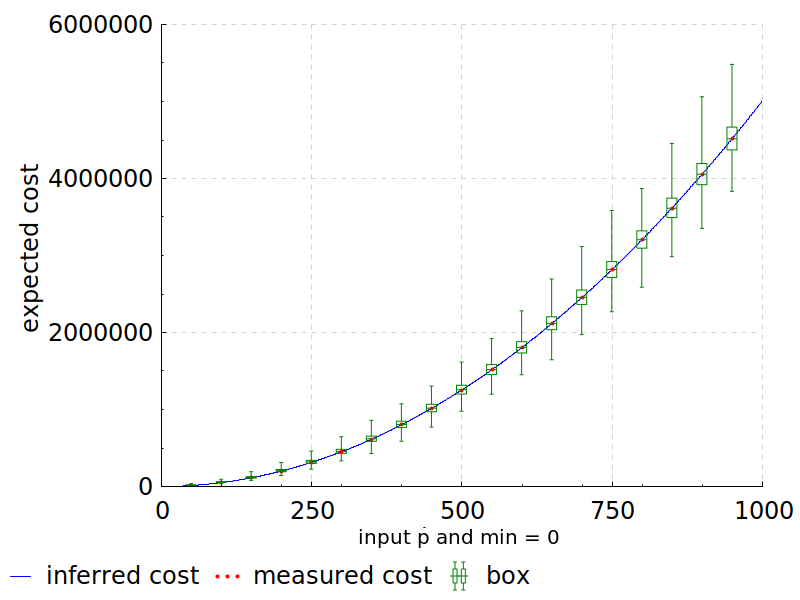
\includegraphics[width=4cm]{Trader.png}}
      \end{center}
    }\only<3->{
      \vspace{1mm}
      \begin{figure}[t]
        \centering
        \begin{tikzpicture}[scale=0.60,baseline=(current bounding box.north)]
          \begin{axis}[
            %
            xlabel={Number of shares},
            xticklabel={\strut$10^{\pgfmathprintnumber{\tick}}$},
            ]

            \addplot[ecoimpbar] table[x=nestings,y=ecoimp]{\tradertimes};
            \addplot[ngobar] table[x=nestings,y=Ngo]{\tradertimes};
            \addplot[wangbar] table[x=nestings,y=Wang]{\tradertimes};

            \legend{\ecoimp,\tool{Absynth},Wang et al};
          \end{axis}
        \end{tikzpicture}
        \caption{Execution times vs sampled shares.}
      \end{figure}
    }
  \end{overlayarea}

  \begin{floating}([xshift=-4mm,yshift=6mm]current page.south east)[south east]
 \begin{codebox}{min,p,n}{6cm}
 while (p > min >= 0) {
   if (Coin($\sfrac{1}{4}$)) {
     p := p + 1
   } else { p := p - 1 };

   n := Uniform(0,$\DRED<3>{\text{\basicstyle{10}}\only<3>{{}^i}}$); $\phantom{{}^i}$
   while (n > 0) {
     consume(p); n := n - 1
   }
 }
\end{codebox}
  \end{floating}
  \end{frame}

    \begin{frame}[t,fragile]
    \frametitle{Coupon Collector [Kaminski et al.'16]}

  \experiment{Coupons}
  {$\norm{n} + \sfrac{1}{2} \norm{n}^2$}{0.195}
  {\notsupported}{}
  {\notsupported}{}

  \vspace{-6mm}
  \begin{overlayarea}{6.5cm}{4cm}
    \begin{center}
      \fbox{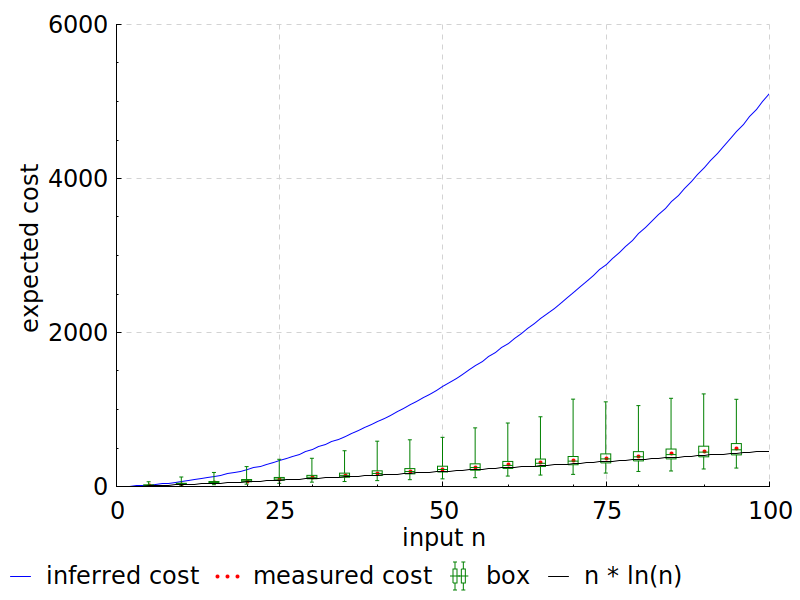
\includegraphics[width=4cm]{CouponCollector.png}}
    \end{center}
  \end{overlayarea}

  \begin{floating}([xshift=-4mm,yshift=6mm]current page.south east)[south east]
\begin{codebox}{coupons,draw,n}{7cm}
 coupons := 0;
 while (0 <= coupons < n) {

   draw := Uniform(1,n);
   if (draw > coupons) {
     coupons := coupons + 1
   }

   consume(1);
}
\end{codebox}
  \end{floating}
\end{frame}

\begin{frame}[t,fragile]
  \frametitle{Nested Loops}

  \experiment{Nest-3}
  {$2\norm{2+n} + 16\norm{n}^2+64\norm{n}^3$}{0.068}
  {$2\norm{1+n} + 4\norm{1+n}^2 + 8\norm{1+n}^3$}{5.130}
  {\fail}{}


  \vspace{-10mm}
  \begin{overlayarea}{6.5cm}{4.5cm}
    \vspace{1mm}
    \begin{center}
      \begin{tikzpicture}[scale=0.50,baseline=(current bounding box.north)]
        \begin{axis}[
          %
          xlabel={Number $N$ of nestings},
          % xticklabel={\strut$10^{\pgfmathprintnumber{\tick}}$},
          ]

          \addplot[ecoimpbar] table[x=nestings,y=ecoimp]{\nesttimes};
          \addplot[ngobar] table[x=nestings,y=Ngo]{\nesttimes};
          \addplot[wangbar] table[x=nestings,y=Wang]{\nesttimes};

          \legend{\ecoimp,\tool{Absynth},Wang et al};
        \end{axis}
      \end{tikzpicture}
    \end{center}
    \end{overlayarea}
    
  \begin{floating}([xshift=-4mm,yshift=6mm]current page.south east)[south east]
\begin{codebox}{n,x}{6cm}
NEST(0) := skip


NEST(N + 1) := {
  x : = m
  while (x > 0) {
    x := x + Uniform(-2,1);
    consume(1);

    NEST(N)
  }
}
\end{codebox}
  \end{floating}
\end{frame}

  \begin{frame}
    \frametitle{Conclusion}

    \begin{enumerate}
    \item
      a novel \DGREEN{expected cost analysis of probabilistic, imperative programs}
      \smallskip
      \begin{itemize}
      \item \DGREEN{modular}: analysis bottom-up; inside out \smallskip
      \item \DGREEN{local}: focus on program fragments significantly simplifies constraint extraction and solving
      \end{itemize}
      \bigskip
    \item
      proven sound in terms of a novel \DBLUE{operational semantics}
      \bigskip
    \item \DRED{fully automated implementation \ecoimp}
    \end{enumerate}
  \begin{center}
      \small$\mparbox[c]{1cm}{\text{\DGREEN{\url{http://www-sop.inria.fr/members/Martin.Avanzini/software/eco-imp/}}}}$
    \end{center}
  \end{frame}

\section{Thank You for Your Attention!}

\bibliographystyle{plain}
\bibliography{references}
\end{document}



